\graphicspath{{litreview/fig/}}

\chapter{Literature Review}
\label{chap:litreview}


\section{Theory and applications of superconductivity}
In order to understand and apply the methods described in \cite{fluxNoiseSquidsStevenAnton} one must first understand the basic theory behind superconductivity as well as some examples of how this theory is used in practice.

\subsection{Superconductivity}
Since the first discovery of superconductivity a couple of successfully theories have been put forth to explain the phenomenon. The London theory is a framework that describes the qualitative behaviour of superconductors and correctly describes perfect diamagnetism and zero resistance but fails to explain the effect on a microscopic level \cite{Golubov_1998}. The London equations (equation \ref{eq:london1} and equation \ref{eq:london2}) \cite{Tinkham_2015} is an addition to Maxwell's equations.
\begin{equation}
    E = \frac{\partial}{\partial t}(\Lambda J_s)
    \label{eq:london1}
\end{equation}
\begin{equation}
    h = -c \nabla\times (\Lambda J_s)
    \label{eq:london2}
\end{equation}
Here $\Lambda$ is a phenomenological parameter determined through experimentation. \par BCS theory put forth a microscopic model of superconductors and explains the phenomenon as a quantum mechanical effect. The details are out of scope for this project but on a crude, qualitative level BCS theory can be explained by the pairing of electrons in the crystal lattice of the superconductor allowing them to be considered one particle. These particles are known as cooper-pairs. At extremely low temperatures the formation of these cooper pairs are energetically favourable \cite{Feynman_Leighton_Sands_2013}. Electron pairs in this state can flow through the superconductor unimpeded.

\subsection{The Josephson junction}
In superconducting electronics the active component is the Josephson junction \cite{Duzer_1999_Princip_Super}. The Josephson junction refers to a situation where two superconductors are connected through a thin non-conductive barrier. If this barrier is thin enough one can observe what is known as the Josephson effect. This phenomenon is can be explained by considering the effect of quantum tunnelling of cooper pairs through the non-conductive boundary. For a sufficiently large barrier one can express the ensemble average wave function in each superconductor independently\cite{Duzer_1999_Princip_Super}:
\begin{equation}
    \Psi = |\Psi(\Vec{r})| \exp{\{i\theta(\Vec{r})\}}
    \label{eq:ensembleWave}
\end{equation}
This is due to the fact that it is energetically favourable for cooper pairs in proximity to one another to lock phases \cite{Duzer_1999_Princip_Super} allowing one to express a large collection of these cooper pairs as one ensemble wave function. The idea that it is energetically favourable for cooper-pairs in proximity to one another extends to the situation where the superconductors are separated by an insulating boundary. When the barrier is sufficiently small the energy of the system can be reduced by the coupling of wave functions in their respective superconductors \cite{Duzer_1999_Princip_Super}. This results in cooper-pairs being able to move across the boundary without energy loss. Following the derivation in \cite{Feynman_Leighton_Sands_2013} one can describe the system behaviour using Schrödinger's equation when a voltage is applied to the junction \cite{Feynman_Leighton_Sands_2013}: 
\begin{equation}
    i\hbar \frac{\partial\Psi_1}{\partial t} = U_1\Psi_1 +K\Psi_2 
    \label{eq:shrod1}
\end{equation}
\begin{equation}
    i\hbar \frac{\partial\Psi_2}{\partial t} = U_2\Psi_2 +K\Psi_1
    \label{eq:shrod2}
\end{equation}
Here $U_1 = qV/2$ and $U_2 = -qV/2$ \cite{Feynman_Leighton_Sands_2013} refer to the energy of the two wave functions and $K$ refers to the coupling energy between each wave function. By taking \ref{eq:ensembleWave} and setting $|\Psi(\Vec{r})|$ equal to $\sqrt{\rho}e^{i\theta}$, where $\rho$ refers to the cooper pair density in the super conductor. One can substitute the result into equations \ref{eq:shrod1} and \ref{eq:shrod2}. From this substitution one can find that the rate of change of electron density on either side of the junction to be described by the following equation \cite{Feynman_Leighton_Sands_2013}:

\begin{equation}
    \dot\rho_1 = \frac{2}{\hbar}K\sqrt{\rho_1\rho_2}sin(\delta)
    \label{eq:charge_dens}
\end{equation}

Where $\rho_1$ is the electron density on one side of the junction. The rate of change of charge on the other side of the junction is simply $\dot\rho_2 = -\dot\rho_1$\cite{Feynman_Leighton_Sands_2013}. The rate of change of charge is the current and therefore the current through the junction can be expressed as follows \cite{CPRJJ}:

\begin{equation}
    I = I_0sin(\theta_2 - \theta_1)
    \label{eq:joseph}
\end{equation}

Equation \ref{eq:joseph} is known as the current-phase relation of the DC Josephson effect.
The phases of the currents on each side of the boundary is described by equation \ref{eq:phasedif} \cite{Feynman_Leighton_Sands_2013}.

\begin{equation}
    \dot\theta_2 - \dot\theta_1 = \frac{qV}{\hbar} = \dot\delta
    \label{eq:phasedif}
\end{equation}

Integrating on both sides yields equation \ref{eq:phaseVoltage}:

\begin{equation}
    \delta(t) = \delta_0 + \frac{q}{\hbar}\int V(t) dt
    \label{eq:phaseVoltage}
\end{equation}

It is important to note that \ref{eq:joseph} is only valid for a limited number of cases and the actual current-phase relation is often more complicated \cite{CPRJJ}. The applications of equation \ref{eq:joseph} is limited to analysing analogue and digital devices based on Josephson junctions \cite{CPRJJ}.

\begin{figure}[h]
    \centering
    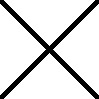
\includegraphics[width=0.1\linewidth]{JJ}
    \label{fig:JJ}
    \caption{The circuit symbol for a Josephson junction}
\end{figure}
\subsubsection*{The RCSJ model}
The phase-current and phase-voltage relation makes the assumption of a perfect Junction. This assumption is inaccurate and as such the RCSJ model is used to more accurately model the behaviour of a junction \cite{Tinkham_2015}. The resistively and capacitively shunted junction is a simple model used to describe the dynamics of a junction. As the name implies it consists of a resistor ($R$), capacitance ($C$) and a Josephson current ($I_s$). In a non-ideal junction a displacement current flows between the two superconductors. This displacement current is modelled by the capacitor. The resistive element models the effect of quasi-particle tunnelling across the boundary \cite{Duzer_1999_Princip_Super}. Figure \ref{fig:RCSJ} depicts the RCSJ model. 
\begin{figure}[H]
    \centering
    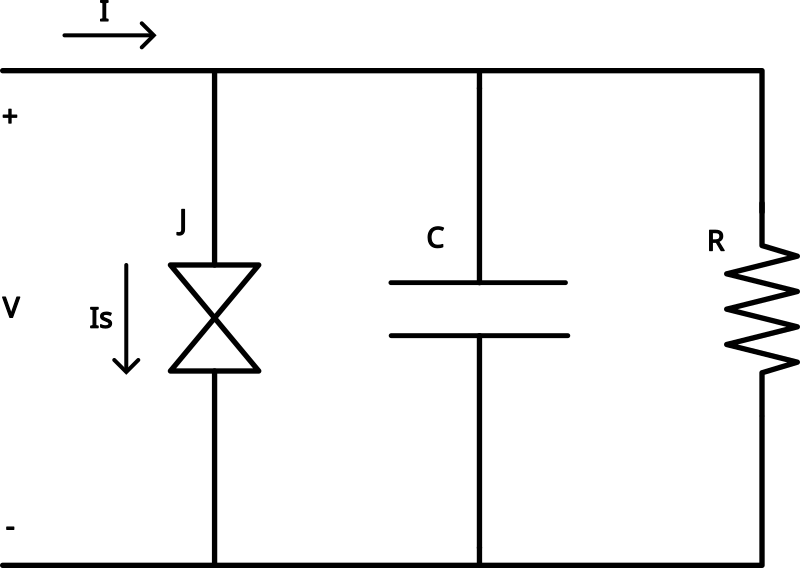
\includegraphics[width=0.5\linewidth]{RCSJ}
    \caption{The circuit schematic of an RCSJ model.}
    \label{fig:RCSJ}
\end{figure}
To derive the current-voltage relation of an RCSJ model one can express the voltage across the parallel components as a function of the current flowing into the junction: 
\begin{equation}
    I = I_csin(\delta)+C\frac{dV}{dt}+\frac{V}{R}
    \label{eq:RCSJ}
\end{equation}
Equation \ref{eq:RCSJ} can be re-written using equation \ref{eq:phaseVoltage}. The resulting equation is a second-order non-linear, inhomogeneous differential equation for which analytical solutions are not available. For the simple case when $C=0$ a differential equation of the form of equation \ref{eq:C0} can be obtained.
\begin{equation}
    K = \frac{d\varphi }{d\tau} + sin(\varphi)
    \label{eq:C0}
\end{equation}
This equation can be integrated directly using separation of variables and a Weierstrass substitution \cite{Duzer_1999_Princip_Super}. The resulting equation describes the dynamics of the phase shift for a constant input current. The frequency of the current through the junction is determined by the dynamics of the phase. The period of the phase-dynamics is the Josephson frequency. Using the Josephson frequency relation \cite{Duzer_1999_Princip_Super},
\begin{equation}
    \omega = \frac{q}{\hbar}V
    \label{eq:JosephsonFreq}
\end{equation}
as well as the period of the equation for the phase, we find the time average voltage of the junction to be \cite{Duzer_1999_Princip_Super}:
\begin{equation}
    V = 
    \begin{cases}
        0 & \quad\text{for } I \le I_c\\
        I_cR[(\frac{I}{I_c})^2-1]^\frac{1}{2} & \quad\text{for } I > I_c\\
    \end{cases}
    \label{eq:IVCHAR}
\end{equation}

\subsection{SQUID's}
An application of the Josephson effect is the superconducting quantum interference device (SQUID). In essence a SQUID refers to a superconducting ring that contains one or more Josephson junction. This interference effect is analogous to interference one might encounter in the field of optics \cite{DCSQUIDoriginalPaper}. The SQUID is a highly sensitive device that can in some cases measure fields as weak as $5\times 10^{-14} T$ \cite{Drung2016NBSQUIDS}.

\subsubsection*{Flux quantisation}
To understand the basic operation of a SQUID, one must first understand the concept of flux quantisation. To do so we consider a superconducting ring in the presence of a uniform magnetic field. The ring is superconducting, so it exhibits the Meissner effect and thus the current density inside the ring is zero. Recall that the flux through a ring is:
\begin{equation}
    \Phi = \oint \Vec{A} \cdot d\Vec{s}
\end{equation}
Now consider the equation for the current density in a superconductor \cite{Feynman_Leighton_Sands_2013}: 
\begin{equation}
    \Vec{J} = \frac{\rho\hbar}{m}(\nabla\theta - \frac{q\Vec{A}}{\hbar})
    \label{eq:current}
\end{equation}
The current density inside the ring in the superconducting state is zero so equation \ref{eq:current} becomes:
\begin{equation}
    \nabla\theta = \frac{q}{\hbar}\Vec{A}
    \label{eq:zeroCur}
\end{equation}
Integrating on both sides around a curve deep inside the superconductor such that the assumption that the current density is zero holds we can express equation \ref{eq:zeroCur} as:
\begin{equation}
    \oint\nabla\theta\cdot d\Vec{s} = \frac{q\Phi}{\hbar}
    \label{eq:intCurrent}
\end{equation}
Recognizing $\nabla\theta$ as vector field with potential function $\theta$, we can simply write the left-hand side of equation \ref{eq:intCurrent} as $\theta(\Vec{r_1}) - \theta(\Vec{r_1})$. One might assume that the left-hand side of the equation \ref{eq:intCurrent} must be equal to zero. This is incorrect because the absolute phase, meaning the potential function $\theta$ cannot be determined and can only be determined up to some constant because the gradient of the scalar potential function will take any constant to zero. Therefore, the phase can only be determined relative to some point. According to \cite{Feynman_Leighton_Sands_2013} the only limitation we can place on the phase of the wave function is that the wave function must be singularly valued. This is intuitively understood as the fact that a particle cannot have two different amplitudes to be in a certain quantum state as that would imply that it has two probabilities associated with the exact same quantum state \cite{Feynman_Leighton_Sands_2013}. From equation \ref{eq:ensembleWave} one can conclude that the phase can change by any integer multiple of $2\pi$ as this results in the exact same wave function. Equation \ref{eq:intCurrent} then becomes:
\begin{equation}
    2\pi n = \frac{q\Phi}{\hbar}
    \label{eq:fluxQuant}
\end{equation}
Clearly equation \ref{eq:fluxQuant} implies that the flux through the superconducting loop must be quantized as $n$ can only take on integer values.

\subsubsection*{The DC SQUID}
Spurred on by developments in reliable manufacturing processes of Josephson junctions the DC SQUID has become the dominant device in the field of niobium based sensors \cite{Drung2016NBSQUIDS}. The initial discovery of the DC SQUID by \cite{DCSQUIDoriginalPaper} in 1964 came shortly after the discovery of the Josephson junction in 1962 \cite{JOSEPHSONJUNCTION}. The simplest realisation of the DC SQUID consists of two Josephson junctions connected in parallel as depicted in figure \ref{fig:squidFig}.

\begin{figure}[h]
    \centering
    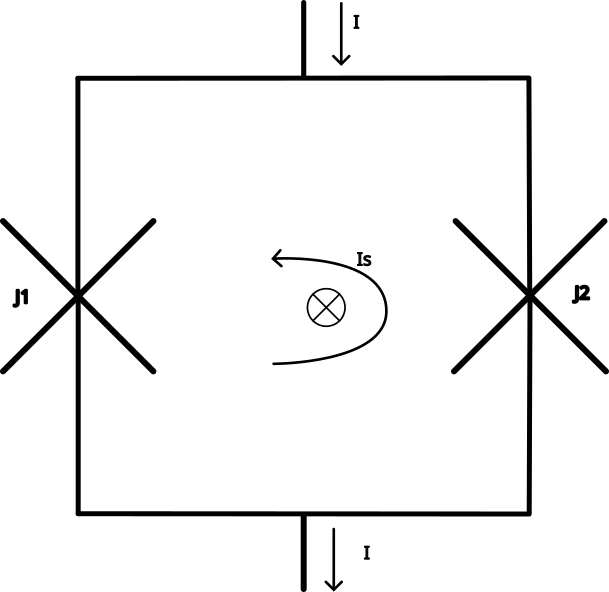
\includegraphics[width=0.3\linewidth]{SQUID}

    \caption{A circuit schematic depicting the configuration of a simple DC SQUID. The current $I$ is the bias current and the current $I_s$ is the screening current developed by an external magnetic field}
    \label{fig:squidFig}
\end{figure}

A relationship between the current and the flux through the loop of the SQUID would like to be derived. The current through each Josephson junction is denoted as $I_1$ and $I_2$ for junction 1 and 2 respectively. From figure \ref{fig:squidFig} one can easily see that there are 2 possible paths through the SQUID. Following the derivation of \cite{Feynman_Leighton_Sands_2013} one can write the change in phase through each branch of the squid using equations \ref{eq:PhaseChange1} and \ref{eq:PhaseChange2} \cite{Feynman_Leighton_Sands_2013}.

\begin{equation}
    \Delta\theta_{1} = \theta_1 + \frac{2q_e}{\hbar}\int_{\text{left branch}} \Vec{A}\cdot d\Vec{s}
    \label{eq:PhaseChange1}
\end{equation}

\begin{equation}
    \Delta\theta_{2} = \theta_2 + \frac{2q_e}{\hbar}\int_{\text{right branch}} \Vec{A}\cdot d\Vec{s}
    \label{eq:PhaseChange2}
\end{equation}
Where $\theta_1$ and $\theta_2$ is the change in phase across their respective junctions. Similarly, $\Delta\theta_1$ and $\Delta\theta_2$ refer to the change in phase through the left and right branch respectively. As previously discussed, the integral of the phase gradient around a closed loop must be an integer multiple of $2\pi$. As a consequence, subtracting equation \ref{eq:PhaseChange2} from \ref{eq:PhaseChange1} must yield $2\pi n$. Using equation \ref{eq:intCurrent} we derive equation \ref{eq:loopInt}.

\begin{equation}
    \theta_2  = \theta_1 - 2\pi n + \frac{2q_e}{\hbar}\Phi
    \label{eq:loopInt}
\end{equation}

Using equation \ref{eq:joseph}, \ref{eq:loopInt} and a KCL at the top or bottom node, the relation between the current going into the loop and the flux through the loop is derived and equation is found. Here the $2\pi n$ term can be neglected as a $2\pi n$ shift in phase does not change the value of the function. 

\begin{equation}
    I = I_2sin(\theta_2) + I_1sin(\theta_2 - \frac{2q_e}{\hbar}\Phi)
    \label{eq:squidI}
\end{equation}

Equation \ref{eq:squidI} describes the current phase characteristic of a 2 junction SQUID. Figure \ref{fig:cv} shows the flux-voltage and current-voltage relationships. 
\begin{figure}[H]
    \centering
    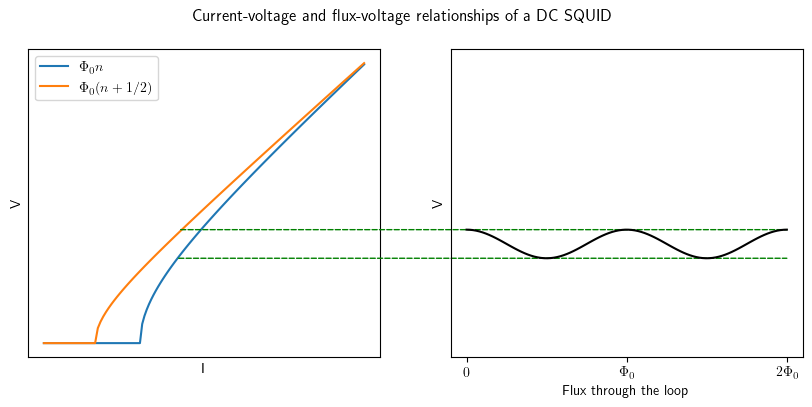
\includegraphics[width=0.7\linewidth]{cvfv}
    \caption{A figure that depicts both the current-voltage (left) and flux-voltage (right) relationship for a DC SQUID. }
    \label{fig:cv}
\end{figure}
It is worth pointing out the mechanism through which flux is quantized in the SQUID loop. When an external field is applied to the washer a screening current begins to flow around the loop to oppose the applied field. The magnitude of the current is determined by the loop inductance. Assuming that the applied flux density is constant throughout the hole in the loop, the magnetic flux generated by the screening current is $\Phi_s = LI_s$. The total flux in the loop is $\Phi_{\text{ext}} + \Phi_{s} = n\Phi_0$. If applied flux is less than $\frac{\Phi}{2}$ the screening current flows to oppose the build up of flux in the loop by ensuring that $\Phi_s = -\Phi_{\text{ext}}$ and thus the total flux in the loop is 0. When the applied flux increases to $\frac{\Phi}{2}$ the flux state of the loop changes and the screening current changes direction \cite{Drung2016NBSQUIDS} to ensure that the total flux in the loop is $\Phi_0$. If the external flux is further increased the flux induced by the screening current decreases from $\frac{\Phi_0}{2}$ to $0$ such that the total flux in the loop remains $\Phi_0$. The trend continues as the external field strength is increased. Because of this mechanism the critical current and voltage-flux characteristics of the SQUID always has a period of $\Phi_0$ \cite{SQUIDhandbook}. As pointed out by \cite{Drung2016NBSQUIDS}, this allows the SQUID to be automatically calibrated as 1 period corresponds to 1 flux quantum in the loop.

\subsection{Practical DC SQUIDS and design considerations}

\subsubsection*{The resistively shunted junction}
Practical realisation of a DC SQUID requires that the designer connect shunt resistors to each junction \cite{Drung2016NBSQUIDS}. This is done such that the system is strongly over damped \cite{SQUIDhandbook}. In the context of the discussion on the I-V characteristics  of the Josephson junction the addition of the shunt resistors correspond to the effect of the junction capacitance becoming negligible. In the absence of a shunt resistor the I-V characteristics of a Josephson junction has hysteresis \cite{Drung2016NBSQUIDS}. 

\subsubsection*{Effective Area and Inductance}
Two important quantities for the design and analysis of SQUID sensors are the effective area and the SQUID inductance. The effective area of a SQUID washer is defined as \cite{SQUIDhandbook}:

\begin{equation}
    A_{\text{eff}} = \frac{\Phi_s}{B_a}
    \label{eq:effArea}
\end{equation}
In equation \ref{eq:effArea} $\Phi_s$ refers to the flux coupled into the SQUID loop as a result of an applied magnetic field $B_a$. The effective area is typically higher than the geometric area of the washer hole due to the Meissner effect \cite{Drung2016NBSQUIDS}. As will be shown in the next section there is a limit on the inductance of a SQUID loop and by extension a limit on how large one can make a SQUID. Critically, the field sensitivity is inversely proportional to the effective area. The magnetic field noise is inversely proportional to the geometric area of the hole in the SQUID loop. The design then comes down to creating a SQUID loop that maximises the effective area but minimizes the actual area of the SQUID loop to keep the SQUID loop inductance and thus the field noise to a minimum \cite{SQUIDhandbook}.

\subsubsection*{The uncoupled SQUID}
Below is an example of an uncoupled DC SQUID structure. 
\begin{figure}[h]
    \centering
    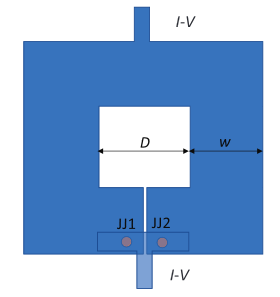
\includegraphics[width=0.4\linewidth]{UncoupledSQUID}
    \caption{A diagram of a practical uncoupled DC SQUID structure \cite{DCSQUIDdesignImage}}
    \label{fig:UncoupledSQUID}
\end{figure}
The uncoupled SQUID is the simplest of designs as it only consists of a single superconducting loop with 2 resistively shunted Junctions. The SQUID characteristics are determined by the loop inductance, critical current, shunt resistance and parasitic junction capacitance \cite{Drung2016NBSQUIDS}. Design involves choosing the optimal set of these parameters to satisfy the design requirements. This is often not a trivial task due to the non-linear nature of the equations describing the behaviour of the Josephson junction and by extension the DC SQUID. Through extensive simulation a number of key design parameters have been identified \cite{Drung2016NBSQUIDS}. The first of which is described by equation \ref{eq:NoisePar} and is referred to as the noise parameter \cite{SQUIDhandbook}. 
\begin{equation}
    \Gamma = \frac{2\pi k_bT}{\Phi_0I_c}
    \label{eq:NoisePar}
\end{equation} 
The noise parameter is the quotient of the thermal energy and the Josephson coupling energy \cite{SQUIDhandbook}. It has the effect of an apparent reduction in the critical current of a junction at low voltages \cite{Drung2016NBSQUIDS}. \newline
The second design consideration is the quality or "Q" factor. For currents the phase shift induced by the Josephson junction can be interpreted as an inductor \cite{SQUIDhandbook}. Under this approximation it is clear to see how the combination of the shunt capacitance and junction create an RC resonator. As pointed out by \cite{Drung2016NBSQUIDS} it is often desirable to keep the quality factor of resonating circuits in non-linear systems close to unity. This leads to the next design rule \cite{SQUIDhandbook}:
\begin{equation}
    \beta_c = Q_j^2 = 2\pi I_cR^2\frac{C}{\Phi_0} \approx 1
    \label{eq:QFACT}
\end{equation}
This parameter is largely controlled by designer by tuning the shunt resistance.\newline
The next design rule sets a constraint on the choice of L (the inductance of the SQUID washer). The magnitude of the screening current in the loop is related to the applied flux through the inductance of the SQUID washer. Increasing the SQUID loop inductance results in a smaller screening current induced in the loop to keep the flux in the loop at an integer multiple of the flux quantum. This leads to a smaller modulation depth of the critical current and by extension the modulation depth of the voltage flux characteristic of the SQUID \cite{Drung2016NBSQUIDS}. For this reason it is generally better to keep the inductance of the SQUID washer low. Simulations have shown that for very low inductances the SQUID noise increases, so a compromise is in order \cite{Drung2016NBSQUIDS} leading to the next design rule: 
\begin{equation}
    \beta_L = \frac{2LI_c}{\Phi_0} \approx 1
    \label{eq:SQUIDmodDepth}
\end{equation}

\section{Noise in SQUIDS}
\label{sec:noiseInSquids}
The importance of understanding, modelling and predicting the noise energy of a SQUID design cannot be understated. A reduction in flux noise necessarily increases the sensitivity of a SQUID system. As reported by \cite{LowNoiseGrad} a typical commercially available SQUID system can achieve magnetic field resolutions of $5 \si{fT/Hz}$. Experimental results suggest that the current consensus on the origin of white noise is in agreement with the theory, that is the origin of the noise is known. The theory explains the white noise as thermal noise and the statistical properties are usually well known \cite{Drung2016NBSQUIDS} \cite{SQUIDhandbook}. For frequencies greater than about $10 - 100\si{Hz}$ the thermal noise dominates. Below $10 - 100\si{Hz}$ the so called $1/f$ noise dominates \cite{DCSQUIDdesignImage}. Unlike thermal noise no consensus has been found on the origin of $1/f$ noise. According to \cite{SQUIDhandbook}, in the fields of biomagnetism and geophysics the low noise properties of SQUIDS must extend to frequencies below $1\si{Hz}$. Furthermore, \cite{QubitPerf} reports the primary cause of decoherence in frequency tuneable quits is the so called $1/f$ flux noise, once again highlighting the important role $1/f$ flux noise has. The low frequency noise power spectral density consists of 2 components (excluding white noise). It consists of critical current fluctuations as well as a flux like term \cite{FluxNoiseCol,fluxNoiseSquidsStevenAnton}. The critical current noise has been shown to be temperature dependant and is well described by existing theory. It is the objective of this project to model the excess flux noise. In the interest of simplicity, the $1/f$ noise discussed hereafter refers specifically to the excess $1/f$ flux noise and not to the critical current noise. 


\subsection{1/f flux noise}
\subsubsection*{The random telegraph signal}
A simple model that gives rise to a 1/f like spectrum is that of the random telegraph signal (RTS). A simple 2 state stochastic process with a mean time in each state of $\tau $ seconds has the following spectral density \cite{fluxNoiseSquidsStevenAnton}: 
\begin{equation}
    S_{\text{RTS}}(f) = \frac{1}{4\pi}\frac{2/\tau}{(2\pi f)^2+(2/\tau)^2}
    \label{eq:RTSPSD}
\end{equation}
If we assume a number of IID random telegraph processes then the resulting distribution is the sum of each individual distribution. Furthermore, if the distribution of each $\tau$ for all processes varies with $1/\tau$ then you get a distribution that scales with $1/f$ \cite{fluxNoiseSquidsStevenAnton}. 
\subsubsection*{The properties of flux noise in SQUID's}
Although there is no consensus on the exact origin of $1/f$ noise many agree that the origin of the excess noise at low frequencies is due to randomly reversing of magnetic moments distributed thinly on the surface of a super conductor \cite{FluxNoiseCol}. As \cite{FluxNoiseCol} reports the noise has a power spectral density of the form of equation \ref{eq:PSDnoise}.
\begin{equation}
    S_\Phi(f) = \frac{A}{f^\alpha}
    \label{eq:PSDnoise}
\end{equation}
The parameter A is insensitive to the geometry and materials of the substrate \cite{fluxNoiseSquidsStevenAnton}. The parameter $\alpha$ is the slope of the noise on a log-log plot. In \cite{SurfaceSpinOrig} the authors propose that the origin of magnetic moments on the surface of the superconductor can be attributed to $O_2$ molecules absorbed on the surface. In \cite{OriginAndReductionOf1/fNoise} the authors provide further supporting evidence to the claims of \cite{SurfaceSpinOrig} by investigating the effect of surface treatments on low frequency flux noise. They found that surface treatments as well as a better sample vacuum environment led to significant improvement in low frequency flux noise. Experimental results suggest the spin density on the surface of the superconductor to be $5\times10^{17}m^{-2}$. According to \cite{fluxNoiseSquidsStevenAnton} various authors have characterized the noise due to surface spins by calculating the mean square flux noise ($\langle \Phi^2\rangle $). The authors make use of a model where spins are independently and identically distributed with each spin having a magnetic moment equal to the Bohr magneton ($\mu_B$). The results correlated with experimental evidence as it conformed to the properties of the power spectral density one expects from the low frequency flux noise \cite{fluxNoiseSquidsStevenAnton}. Specifically, the models conformed to the property that the magnitude of the flux noise is a weak function of the geometry of the SQUID.

\subsubsection*{Flux noise measurements}
This project will be tested against recorded flux noise measurements. The critical current will not be accounted for, so it is important that the practical data used for comparison is consistent with this assumption. In \cite{FluxNoiseCol} the authors cooled various SQUID's to millikelvin temperatures. The authors tested a variety of SQUID loop designs. Each SQUID consisted of a $200 nm$ sputtered niobium layer as well as $200nm$ lead layer separated by an isolation layer made of $500nm$ of silicon oxide. To form the Josephson junctions a $2\times 2 um$ via through the silicon oxide was created. The tunnel barrier was constructed out of niobium-oxide. The authors then measured the noise PSD and fit the measurements to equation \ref{eq:PSDFit} to determine the parameters $A$ and $\alpha$.

\begin{equation}
    S_\Phi(f) = Af^{-\alpha} + C
    \label{eq:PSDFit}
\end{equation}
In equation \ref{eq:PSDFit}, the variable $C$ refers to power spectral density of the frequency independent white noise. The authors tabulated these parameters as well as the inductance and physical dimensions of the SQUID loops.

\subsection{Techniques for predicting mean square flux noise}
\label{subsec:PredictFluxNoise}
The importance of being able to predict the low frequency flux noise in SQUID's has led many to attempt to predict it using the mostly agreed upon model of magnetic defects on the surface of the super conductor.

\subsubsection*{Numerical method by Bialczak et al.}
In the work done by Bialczak et al. \cite{BialczakTestLoop}, the authors describe how they calculate the mean square flux noise due to a random distribution of surface defects on the substrate of the SQUID. Critically, the authors do not make the assumption that defects are confined to the surface of the superconducting film. In this method a test loop is used to represent a surface defect. The test loop is dimensioned such that the product of the area of the loop and the current in the test loop is equal to the Bohr magneton. The authors used FastHenry to calculate the mutual inductance between the SQUID and the test loop. Once the mutual inductance is known, one can simply relate it to the flux coupled into the loop by a single magnetic moment by multiplying the test current by the mutual inductance \cite{BialczakTestLoop}. 
\begin{equation}
    \Phi_s = M(x,y)I
    \label{eq:FluxCoupleBial}
\end{equation}
The method requires a new simulation to be run for each location and orientation of the test loop. This is computationally taxing and severely limits the resolution and accuracy of the calculation \cite{fluxNoiseSquidsStevenAnton}. Despite the heavy computational cost of the method it is fairly general and can easily be extended to different geometries. In theory this method could be used to verify the validity of the theoretical model because, given a powerful enough computer, one could perform an exact simulation, neglecting the error due to meshing, where the test loop is dimensioned such that it is on the order of a single surface defect. The authors found that the results they obtained from their numerical model match best when an areal spin density of $5\times10^{17}\si{m^{-2}}$

\subsubsection*{The analytic method of Koch et al.}
The approach taken by \cite{KochModel} attempts to derive analytic solutions for the mean square low frequency flux noise in a SQUID. In \cite{KochModel} the authors examine a theoretical model where the flux noise is a result of two-level state (TLS) defects in the oxides of the superconducting film \cite{KochModel}. A TLS defect is a microscopic defect that can be described by a two-state quantum system \cite{KochModel}. The defects can in principle be any plausible two state quantum system but in \cite{TLSDefectExplanation} the authors list the following as examples of such defects:
\begin{center}
    \begin{itemize}
        \item Tunnelling atoms \\
        \item Dangling electronic bonds \\
        \item Surface impurities \\
        \item Trapped charges \\
    \end{itemize}
\end{center}
To derive an analytic solution for the mean square flux noise figure one has to make assumptions about the nature of the TLS defects. In \cite{KochModel} the assumption that all defects have a magnetic moment equal to the Bohr magneton, the assumption that defects are uniformally distributed across the surface of the superconducting film and the assumption that the magnetic moments of the defects are randomly orientated is made. \par
We start by recognizing that the mutual inductance between any 2 arbitrarily shaped loops in space is equal. That is the inductance matrix is of the form: 
\begin{equation}
    \begin{bmatrix}
        \lambda_1 \\
        \lambda_2 \\
    \end{bmatrix} 
    = 
    \begin{bmatrix}
        L_1 && M \\
        M && L_2 \\
    \end{bmatrix}
    \begin{bmatrix}
       I_1 \\
       I_2 \\
    \end{bmatrix}
    \label{eq:InductanceMatrix}
\end{equation}
The inductance is a function of the geometry of the problem and is therefore independent of the flux and current terms \cite{Feynman_Leighton_Sands_2013}. If one sets $I_2 = 0$ and $I_1 = I'$ it is easy to solve for the mutual inductance: 
\begin{equation}
    M = \frac{\lambda_2}{I'}
    \label{eq:Mutual2}
\end{equation} 
Doing the same but this time setting $I_1 = 0$ and $I_2 = I'$:
\begin{equation}
    M = \frac{\lambda_1}{I'}
    \label{eq:Mutual1}
\end{equation}
Because $M$ is constant in both equations \ref{eq:Mutual1} and \ref{eq:Mutual2}, $\lambda_1$ must equal $\lambda_2$. This demonstrates the principle of reciprocity. Clearly it does not matter which loop is excited by the current $I'$ the flux remains the same in both cases. This is leveraged by \cite{KochModel} because unlike the method employed by Bialczak et al. \cite{BialczakTestLoop}, the test loop becomes the SQUID washer as the flux coupled into the washer due to a magnetic moment is the same as the flux coupled into the area of a magnetic moment (defined as $\Vec{\mu} = \Vec{S}\cdot I$ where S refers to the vector area) due to a test current in the SQUID washer. \par
For a thin wire of diameter $D$ and loop radius $R$, the magnetic field on the surface and tangent to the circular cross-section of the wire is approximated for a large loop radius by applying the ampere circuital law. We choose a path of integration around the diameter of the wire such that the assumption that the magnetic flux density tangent to the cross-section of the loop is constant can be made. Under these assumptions' equation \ref{eq:BField} is found.
\begin{equation}
    B = \frac{\mu_0I}{\pi D}
    \label{eq:BField}
\end{equation}
Following the law of reciprocity we can express the flux through the loop due to a surface defect randomly orientated on the ring at a position $\Vec{r}$:
\begin{equation}
    \Phi = \Vec{\mu_B}\cdot \frac{B(\Vec{r})}{I} 
    \label{eq:Flux}
\end{equation}
The defects are uniformally distributed, so the number of magnetic moments is simply $\sigma 2\pi^2RD$.

\begin{equation}
    \langle \Phi^2 \rangle = \frac{\mu_B^2 \mu_0^2}{\pi^2 D^2}\cdot\langle (\Vec{a_m}\cdot \Vec{a_\text{bfield}(\Vec{r})})^2\rangle \cdot \text{Surface area of the loop} \cdot \sigma
    \label{eq:MSFN}
\end{equation}
Here $\Vec{a_m}$ is a random unit vector representing the direction the magnetic moment is pointing and $\Vec{a_b(\Vec{r})}$ represents the direction of the b field as a unit vector. Trivially, the expectation of the dot product between a unit vector and a random unit vector in $\mathbb{R}^3$ (assuming the random vector has a uniform distribution) evaluates to $\frac{1}{3}$. Simplifying equation \ref{eq:MSFN} and applying this result equation \ref{eq:MSFNfinal}.

\begin{equation}
    \langle \Phi^2 \rangle = \frac{2\mu_0^2\mu_B^2\sigma R}{3D} 
    \label{eq:MSFNfinal}
\end{equation}
This is the same result as found in \cite{KochModel}. Using the same technique \cite{KochModel} derives the equation for the mean square flux noise in a thin film circular loop of radius $R$ and track width $W$ to be:
\begin{equation}
    \langle \Phi^2 \rangle \approx \frac{2\mu_0^2\mu_B^2}{3}\sigma\frac{R}{W}[\frac{\text{ln}(\frac{2bW}{\lambda^2}) }{2\pi}+ 0.27] 
    \label{eq:ThinFilmMSFN}
\end{equation}
The authors concluded that the standard TLS model incorrectly describes the mechanism through which low frequency 1/f flux noise arises. Despite this conclusion, the analytical methods used by \cite{KochModel} is valuable as the use of the principle of reciprocity is the key to the next method used to calculate mean squared flux noise figures.

\subsubsection*{The numerical method of S.M. Anton et al.}
This method follows on closely from the method employed by \cite{KochModel}. In \cite{fluxNoiseSquidsStevenAnton} the same assumptions are made about the nature of the surface defects as in \cite{KochModel}. This technique takes the analytical method demonstrated by \cite{KochModel} and implements it numerically. To do this \cite{fluxNoiseSquidsStevenAnton} makes use of a superconducting version of FastHenry to compute the current distribution due to a time varying voltage source applied to a test port on the SQUID washer as shown in figure \ref{fig:WASHERSteven}.
\begin{figure}[h]
    \centering
    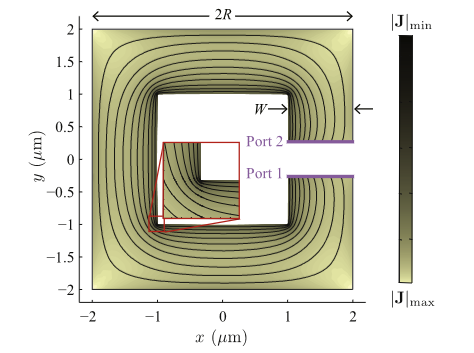
\includegraphics[width=0.5\linewidth]{Washer}
    \caption{A figure produced by \cite{fluxNoiseSquidsStevenAnton} showing the use of a test port on the SQUID washer}
    \label{fig:WASHERSteven}
\end{figure}
The author noted that the time complexity of FastHenry at the time was roughly $\mathcal{O}(N_{\text{seg}})$, where $N_{\text{seg}}$ refers to the number of segments in the mesh. FastHenry did not support a meshing scheme where segments could have varying segment widths \cite{fluxNoiseSquidsStevenAnton}. The author concluded that in order to make the computational load reasonable while still capturing the rapidly varying nature of the current distribution localized to specific regions of the geometry, a new meshing scheme needs to be developed \cite{fluxNoiseSquidsStevenAnton}. To solve this problem the author made use of the software package InductEx to create an optimized mesh where the mesh size is tuned to ensure that the change in current density from one mesh element to the next never exceeds a certain threshold. Once the current distribution is known, the magnetic field on the surface of the SQUID can be calculated using the law of Biot and Savart \cite{fluxNoiseSquidsStevenAnton}:
\begin{equation}
    \Vec{B(\Vec{r})} = \frac{\mu_0}{4\pi}\sum_{\text{sll segments}}[J_n\times\int_{V_n}\frac{\Vec{s}\cdot d\Vec{V}}{|\Vec{s}|^3}]
    \label{eq:BiotSavart}
\end{equation}
The current is assumed to be constant throughout each individual segment so $J_n$ is taken out of the integral in equation \ref{eq:BiotSavart}. This allows the integral to be solved analytically as it only depends on the geometry of a segment and not the current distribution \cite{fluxNoiseSquidsStevenAnton}. Once the magnetic flux density on the surface of the conductor is found, the principle of reciprocity can be used to calculate the mean square flux noise. In \cite{fluxNoiseSquidsStevenAnton} equation \ref{eq:MSFNfromBfield} is listed.
\begin{equation}
    \langle \Phi^2 \rangle = \frac{N\mu_B^2}{3I^2}\langle \Vec{B}^2(\Vec{r}) \rangle
    \label{eq:MSFNfromBfield}
\end{equation}
In conclusion, the author reduces the problem of calculating the mean square flux noise to finding the average magnetic flux density on the surface of the conductor. A detail that is worth mentioning is that the number of spin densities $N$ in equation \ref{eq:MSFNfromBfield} is considered large enough such that one can make a continuum approximation \cite{fluxNoiseSquidsStevenAnton}. It was also found that equation \ref{eq:ThinFilmMSFN} does not agree well with the numerical framework due to assumptions that introduce significant error in the final result.

